\documentclass[a4paper,11pt,oneside]{article}

\usepackage[utf8]{inputenc}
\usepackage[a4paper,top=3cm,bottom=3cm,left=3cm,right=3cm]{geometry}
\renewcommand{\familydefault}{\sfdefault}
\usepackage{helvet}
\usepackage[english]{babel}     %% typographie française
\usepackage[style=numeric,language=english, sorting=none]{biblatex}
\usepackage{parskip}		%% blank lines between paragraphs, no indent
\usepackage[margin=1cm]{caption}%% give long captions a margin
\usepackage{booktabs}           %% typesetting nice tables
\usepackage[pdftex]{graphicx}	%% include graphics, preferably pdf
\graphicspath{ {./images/} }
\usepackage[pdftex]{hyperref}	%% many PDF options can be set here
\pdfadjustspacing=1		%% force LaTeX-like character spacing
\usepackage{amsmath}

\newcommand{\myname}{Tianyao Chen}
\newcommand{\mytitle}{Deep Learning for Detecting Amphoras in Ancient Shipwrecks}
\newcommand{\mysupervisor}{Prof. Dr. Andreas Birk}

\hypersetup{
  pdfauthor = {\myname},
  pdftitle = {\mytitle},
  pdfkeywords = {},
  colorlinks = {true},
  linkcolor = {blue}
}

\addbibresource{Tianyao_Chen_bachelor_thesis.bib}

\begin{document}
  \pagenumbering{roman}

  \thispagestyle{empty}

  \begin{flushright}
    
\includegraphics[scale=0.8]{bsc-logo}
  \end{flushright}
  \vspace*{40mm}
  \begin{center}
    \huge
    \textbf{\mytitle}
  \end{center}
  \vspace*{4mm}
  \begin{center}
   \Large by
  \end{center}
  \vspace*{4mm}
  \begin{center}
    \LARGE
    \textbf{\myname}
  \end{center}
  \vspace*{20mm}
  \begin{center}
    \Large
    Bachelor Thesis in Computer Science
  \end{center}
  \vfill
  \begin{flushleft}
    \large
    Submission: \today \hfill Supervisor: \mysupervisor \\
    \rule{\textwidth}{1pt}
  \end{flushleft}
  \begin{center}
    Jacobs University Bremen $|$ Department of Computer Science and Electrical Engineering
  \end{center}

  \newpage
  \thispagestyle{empty}

  \subsection*{English: Declaration of Authorship}

  I hereby declare that the thesis submitted was created and written
  solely by myself without any external support. Any sources, direct
  or indirect, are marked as such. I am aware of the fact that the
  contents of the thesis in digital form may be revised with regard to
  usage of unauthorized aid as well as whether the whole or parts of
  it may be identified as plagiarism. I do agree my work to be entered
  into a database for it to be compared with existing sources, where
  it will remain in order to enable further comparisons with future
  theses. This does not grant any rights of reproduction and usage,
  however.

  This document was neither presented to any other examination board
  nor has it been published.

  \subsection*{German: Erklärung der Autorenschaft (Urheberschaft)}

  Ich erkläre hiermit, dass die vorliegende Arbeit ohne fremde Hilfe
  ausschließlich von mir erstellt und geschrieben worden ist. Jedwede
  verwendeten Quellen, direkter oder indirekter Art, sind als solche
  kenntlich gemacht worden. Mir ist die Tatsache bewusst, dass der
  Inhalt der Thesis in digitaler Form geprüft werden kann im Hinblick
  darauf, ob es sich ganz oder in Teilen um ein Plagiat handelt. Ich
  bin damit einverstanden, dass meine Arbeit in einer Datenbank
  eingegeben werden kann, um mit bereits bestehenden Quellen
  verglichen zu werden und dort auch verbleibt, um mit zukünftigen
  Arbeiten verglichen werden zu können. Dies berechtigt jedoch nicht
  zur Verwendung oder Vervielfältigung.

  Diese Arbeit wurde noch keiner anderen Prüfungsbehörde vorgelegt
  noch wurde sie bisher veröffentlicht.

  \vspace{20mm}

  Date, Signature

  \newpage

  \section*{Abstract}

  Consider this a separate document, although it is submitted together
  with the rest. The abstract aims at another audience than the rest
  of the proposal. It is directed at the final decision maker or
  generalist, who typically is not an expert at all in your field, but
  more a manager kind of person. Thus, don't go into any technical
  description in the abstract, but use it to motivate the work and to
  highlight the importance of your project.

  (target size: 15-20 lines)

  \newpage
  \tableofcontents

  \clearpage
  \pagenumbering{arabic}

  \section{Introduction}

  % TODO: A general introduction and an outline of the structure.

  \subsection{Motivation}

  \subsubsection{Relevance of Amphoras}

  The name \textit{amphora} is derived from the Greek word \textit{amphoreus}, which literally means "two-handled"
  \cite{harper2001online, twede2002commercial}. It is the combination of two linguistic roots: \textit{amphi}
  (on both sides) and \textit{phoreus} (bearer) \cite{harper2001online, twede2002commercial}. Amphoras (or amphorae)
  were commercially used from 1500 B.C.E. to 500 C.E. to ship products throughout the Mediterranean,
  supplying the ancient Greek and Roman empires \cite{twede2002commercial}. Amphoras were designed to ship large quantities
  of liquid (wine, olives, and oils) and dry products (grain, nuts, and salted fish) \cite{twede2002commercial}.

  Like many measures that are named after the packages, amphoras were also a semi-standard unit of liquid
  measure \cite{twede2002commercial}. A cargo ship's capacity was measured by the number of amphoras it could carry
  instead of by weight \cite{twede2002commercial, cousteau1954fish}.

  The structurally strong egg-like shape and the high volume-to-weight ratio made amphoras very efficient packages
  \cite{twede2002commercial}. Amphoras were by far the most common cargo type in Mediterranean shipwreck analysis;
  more than half of the ships only carried amphoras \cite{twede2002commercial, parker1984shipwrecks}.

  \begin{figure}[ht]
    \begin{center}
      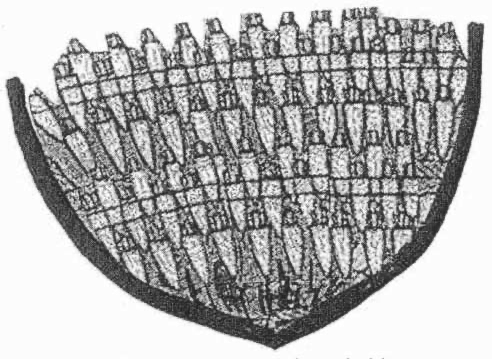
\includegraphics[width=.8\textwidth]{amphora_stowage_aboard_ship.png}
    \end{center}
    \caption{The egg-like shape enabled amphoras to interlock and minimize the waste of space on a ship.
    Source: \cite{twede2002commercial}.}
  \end{figure}

  Amphoras' various shapes and markings - which changed by time, region, producer, contents, and brand
  identity - were used to identify the package status and the different products inside \cite{twede2002commercial}.

  \begin{figure}[ht]
    \begin{center}
      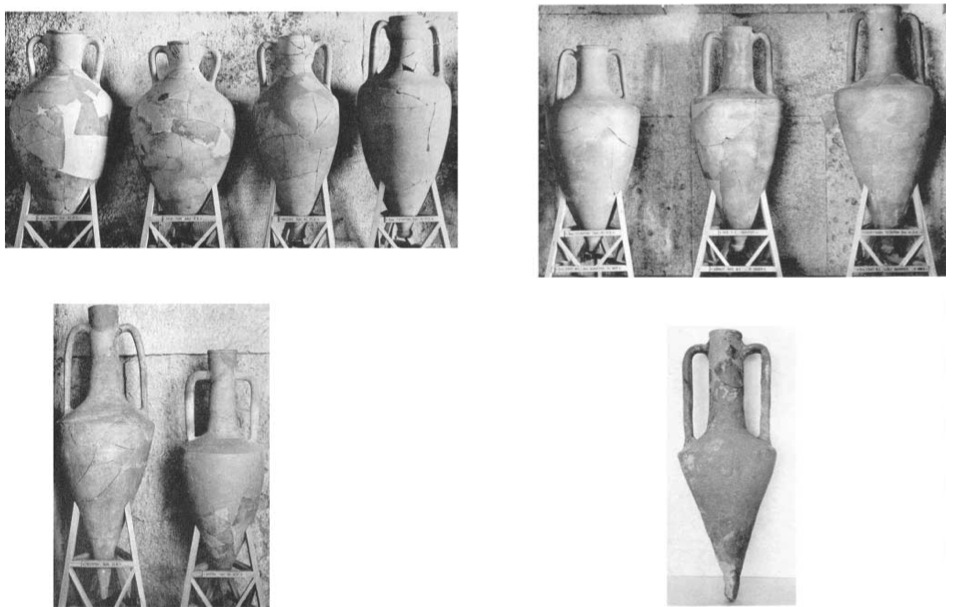
\includegraphics[width=.8\textwidth]{amphora_various_shape.png}
    \end{center}
    \caption{Amphoras have various shapes. Source: \cite{twede2002commercial}.}
  \end{figure}

  Amphoras have great significance in archaeology. They can be used as evidence for the trade patterns throughout
  the Mediterranean \cite{twede2002commercial}. As they were usually discarded at the destination of a trade and have been
  found in shipwrecks, archaeologists have been using them to recreate the transit routes \cite{twede2002commercial}.
  Furthermore, researchers have been able to classify different amphoras, which also helps to date ruins and shipwrecks
  \cite{twede2002commercial}.

  \subsubsection{Computer Vision for Underwater Archaeology}

  \label{sec:112}

  Computer vision is the science of perceiving and understanding the world through images and videos \cite{elgendy2020deep}.
  There have been multiple exciting applications of computer vision, including image classification \cite{rawat2017deep},
  object detection and localization \cite{zhao2019object,liu2020deep}, art generation (neural style transfer)
  \cite{jing2019neural}, image creation with Generative Artificial Networks (GAN) \cite{goodfellow2014generative},
  face recognition \cite{parkhi2015deep}, action and activity recognition \cite{poppe2010survey}, human pose estimation
  \cite{toshev2014deeppose}, and image recommendation system \cite{niu2018neural}.

  However, there is still limited research for the application of computer vision and machine learning in archaeology,
  especially underwater archaeology, compared to other domains \cite{maaten2007computer, qin2015underwater}.
  Computer vision, instead of visual inspection, could be used to automate the detection, assessment, and classification
  of artifacts \cite{maaten2007computer}.

  Underwater computer vision has proven to be challenging, largely due to: 1) the distortion and attenuation caused by
  light propagation in water, 2) the unrestricted natural environment with the abundance of marine life and suspended
  particles, and 3) underwater objects are often broken
  \cite{qin2015underwater, rizzini2015investigation, lu2017underwater, mccarthy20193d}.

  Despite the challenges, computer vision has lower cost \cite{rizzini2015investigation} compared to sonar imagery
  \cite{abu2019statistically} and laser scanning \cite{gordon1992use}. Plus, the increasingly abundant visual data obtained
  through autonomous underwater vehicles (AUVs), unmanned underwater vehicles (UUVs)
  \cite{lu2017underwater, moniruzzaman2017deep}, and seafloor cabled observatories \cite{qin2015underwater} enables us
  to utilize deep learning.

  Furthermore, the research for deep-water shipwrecks is even more limited, mostly due to the lack of information and
  accessibility \cite{drap2015underwater}. However, the need to study deep-water sites are in high demand, as the threats
  to these sites are increasing \cite{drap2015underwater}. One major threat is the new forms of trawling that destroy the
  surface of these sites and interfere with the readability \cite{drap2015underwater}. This means that many
  shipwrecks are likely to be damaged before they can be studied \cite{drap2015underwater}. It is thus crucial to implement
  efficient, accessible, and accurate techniques like deep learning based computer vision to study deep-water shipwrecks.

  \subsection{Deep Learning}

  Machine learning is the class of algorithms that allow computers to learn and improve from data instead of being
  explicitly programmed \cite{samuel1959some, geron2019hands}. And deep learning is the subfield of machine learning that
  builds artificial neural networks with more than one layer between the input and output layers
  \cite{geron2019hands, burkov2019hundred, zhang2018definition}. Deep learning constructs complex representations by
  combining simpler ones from the previous layers \cite{goodfellow2016deep}.

  \begin{figure}[ht]
    \begin{center}
      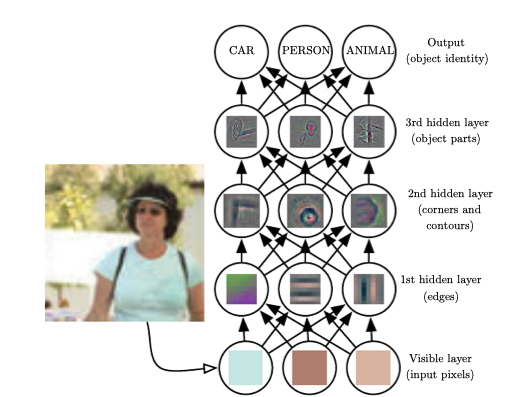
\includegraphics[width=.8\textwidth]{deep_learning.png}
    \end{center}
    \caption{A deep learning system that learns the representations of a person. This is achieved by combining simpler
    features like corners and contours, which are further expressed by combining simpler features like edges. Source:
    \cite{goodfellow2016deep}.}
  \end{figure}

  \subsubsection{Artifical Neural Networks (ANNs)}

  Inspired by the biological neuron, artificial neural networks (ANNs) were first introduced in 1943 using propositional
  logic \cite{mcculloch1943logical}. The artificial neuron activates its single binary output when the number of active
  binary inputs reaches the activation threshold, which enables us to build networks that can perform any logical
  computation \cite{geron2019hands, mcculloch1943logical}.

  \begin{figure}[ht]
    \begin{center}
      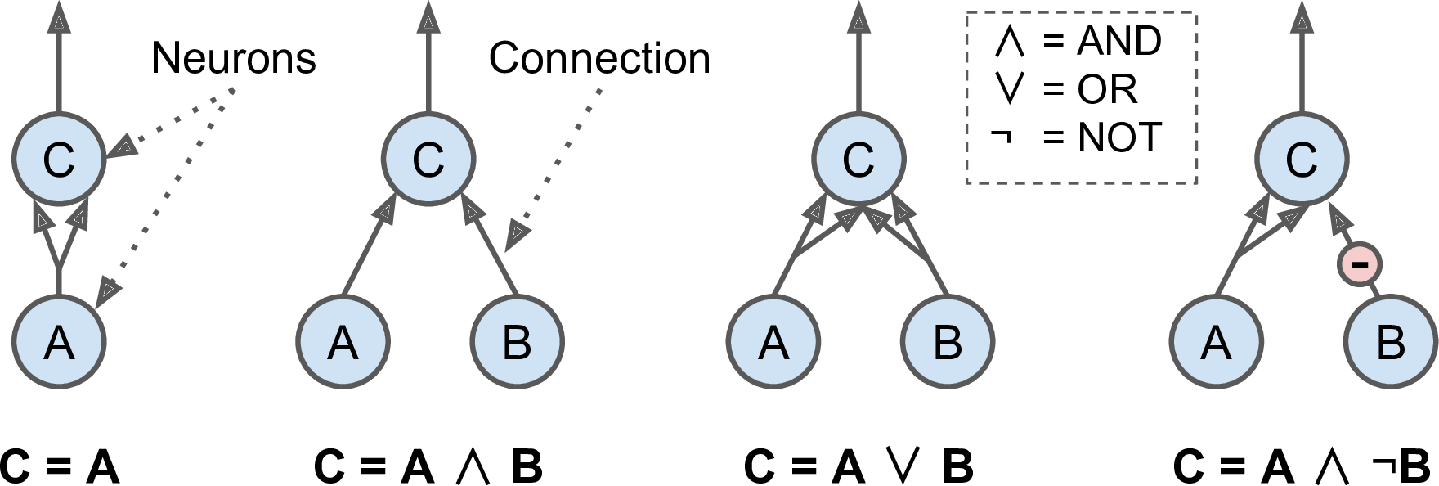
\includegraphics[width=.8\textwidth]{ann_logic_computations.png}
    \end{center}
    \caption{ANNs performing logical computations with the activation threshold of 2. Source: \cite{geron2019hands}.}
  \end{figure}

  Then the Perceptron was introduced in 1957, which is based on a different artificial neuron called threshold logic unit
  (TLU) or linear threshold unit (LTU) \cite{rosenblatt1957perceptron}. The inputs and outputs are numbers instead of
  binary values, and each input has a weight. TLU computes the weighted sum of the inputs and then applies a step
  function like the Heaviside function
  $heaviside (x) =
  \begin{cases}
    0 & x \le 0 \\
    1 & x \geq 0 \\
  \end{cases}$
  \cite{geron2019hands, rosenblatt1957perceptron}.

  \begin{figure}[ht]
    \begin{center}
      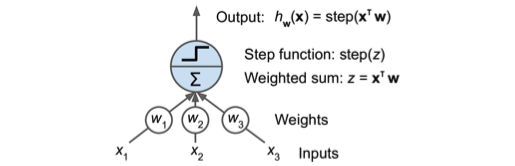
\includegraphics[width=.8\textwidth]{tlu.png}
    \end{center}
    \caption{Threshold logic unit. Source: \cite{geron2019hands}.}
  \end{figure}

  A single TLU can be used for simple linear binary classification, while a layer of TLUs plus a bias neuron form a
  Perceptron capable of multi-output classification \cite{geron2019hands}.

  The outputs of a fully connected layer is computed as follows, where $\mathbf{X}, \mathbf{W}, \mathbf{b}$, and $\phi$
  are respectively the input matrix, weight matrix, bias vector, and activation function:

  $$h_{\mathbf{W,b}}(\mathbf{X}) = \phi(\mathbf{XW} + \mathbf{b})$$

  The Perceptron is trained using a variant of the Herbb's rule \cite{hebb2005organization}, which is famously summarized
  as "neurons wire together if they fire together \cite{lowel1992selection}" \cite{geron2019hands}. However, the Perceptron
  can not learn complex patterns due the linear decision boundary of the output neurons, and it can only make predictions
  based on a hard threshold instead of outputting a class probability \cite{geron2019hands}. To address these limitations,
  the Multilayer Perceptron (MLP) was introduced by stacking multiple Perceptrons.

  \begin{figure}[ht]
    \begin{center}
      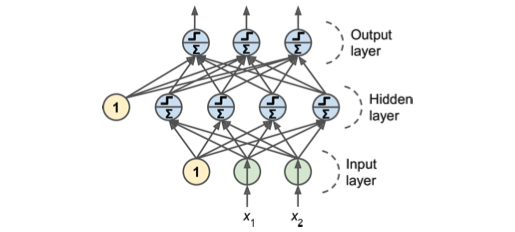
\includegraphics[width=.8\textwidth]{mlp.png}
    \end{center}
    \caption{A Multilayer Perceptron with one hidden layer. Source: \cite{geron2019hands}.}
  \end{figure}

  Backpropagation \cite{rumelhart1985learning} is used to train the MLP, which first makes a prediction and measures the
  error in the forward pass, then measures the error contribution from each connection in the reverse pass, and finally
  tweaks the connection weights to reduce teh error in the Gradient Descent \cite{ruder2016overview} step
  \cite{geron2019hands}. Activation functions like Rectified Linear Unit $ReLU(x) = max(0, x)$ are used to add
  nonlinearity, which theoretically gives a large enough deep neural network the ability to approximate any continuos
  function \cite{geron2019hands}.

  \subsubsection{Convolutional Neural Networks (CNNs)}

  Convolutional Neural Networks (CNNs) were inspired by the brain's visual cortex, and they have been used in computer
  vision since the 1980s \cite{geron2019hands}. We can not simply use a deep neural network with fully connected layers
  for computer vision, as it breaks down for large images due to the huge number of parameters it requires
  \cite{geron2019hands}. CNNs also have successful applications in other domains like recommender systems
  \cite{van2013deep} and natural language processing (NLP) \cite{collobert2008unified}.

  Hubel et al. \cite{hubel1959single, hubel1959receptive, hubel1968receptive} found that many biological neurons have
  a small receptive field, which  means they only react to visual stimuli in a limited region of the visual field
  \cite{geron2019hands}. Some neurons only react to horizontal lines, while others only react to lines with
  different orientations \cite{geron2019hands}. Some neurons have larger receptive fields, and they react to more complex
  patterns formed by lower-level patterns \cite{geron2019hands}.

  Neurons in the first convolutional layer are only connected to pixels in their receptive fields, and neurons in the
  second convolutional layer are only connected to the neurons in a small receptive field in the first layer
  \cite{geron2019hands}. This allows the CNN to concentrate on lower-level features in the first hidden layer, then
  combine them into higher-level features in the second hidden layer, and so on \cite{geron2019hands}.

  \begin{figure}[ht]
    \begin{center}
      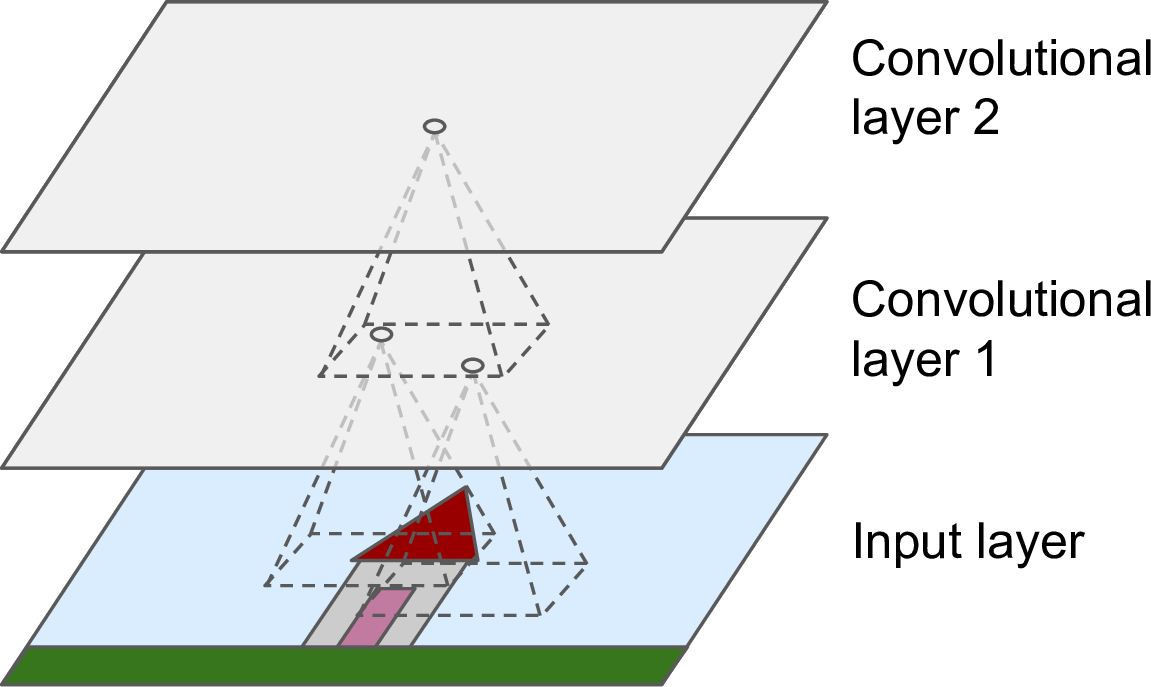
\includegraphics[width=.8\textwidth]{cnn_layers.png}
    \end{center}
    \caption{CNN layers with rectangular receptive fields. Source: \cite{geron2019hands}.}
  \end{figure}

  The filters or convolution kernels, which are learned during training, are neurons' weights that can be presented as
  small images the size of receptive fields \cite{geron2019hands}. For example, a black sqaure with a horizontal white
  line in the middle (a matrix full of 0s except for the central row with 1s) is a filter that only reacts to the central
  row in the receptive field. A layer of neurons with the same filter outputs a feature map, which highlights the parts
  of an image that activate the filter the most \cite{geron2019hands}.

  \begin{figure}[ht]
    \begin{center}
      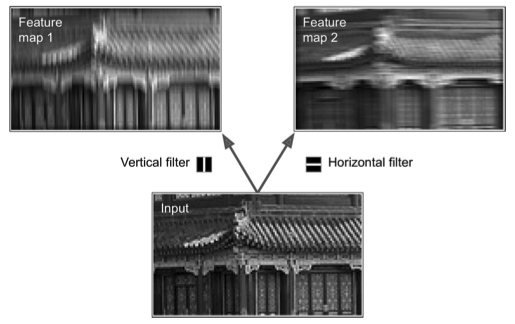
\includegraphics[width=.8\textwidth]{filters.png}
    \end{center}
    \caption{Two feature maps obtained by applying two different filters. Source: \cite{geron2019hands}.}
  \end{figure}

  The pooling layers subsample (i.e. shrink) the input image to reduce the computational load and the number of paramters,
  which also reduces overfitting \cite{geron2019hands}. Plus, pool layers can bring some invariance to small translations,
  rotations, and scaling \cite{geron2019hands}.

  \begin{figure}[ht]
    \begin{center}
      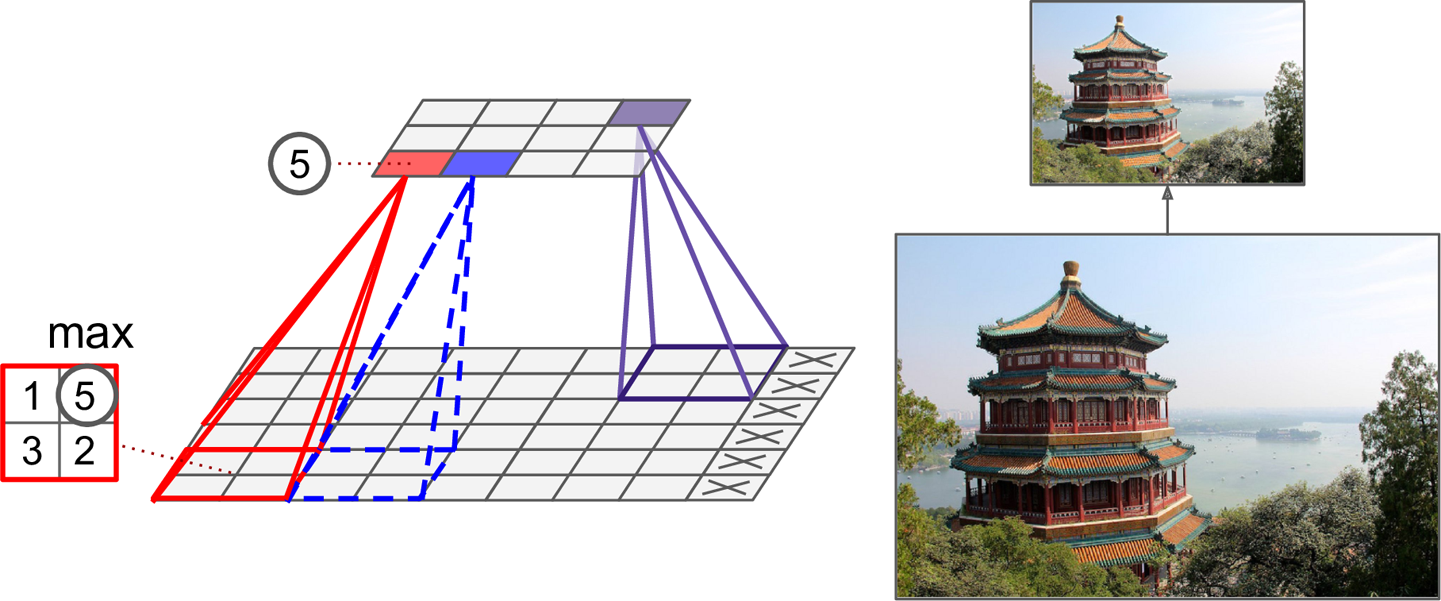
\includegraphics[width=.8\textwidth]{max_pooling.png}
    \end{center}
    \caption{A max pooling layer with a 2 x 2 kernel and stride 2. Only the max value from each receptive field
    gets passed to the next layer. Source: \cite{geron2019hands}.}
  \end{figure}

  \begin{figure}[ht]
    \begin{center}
      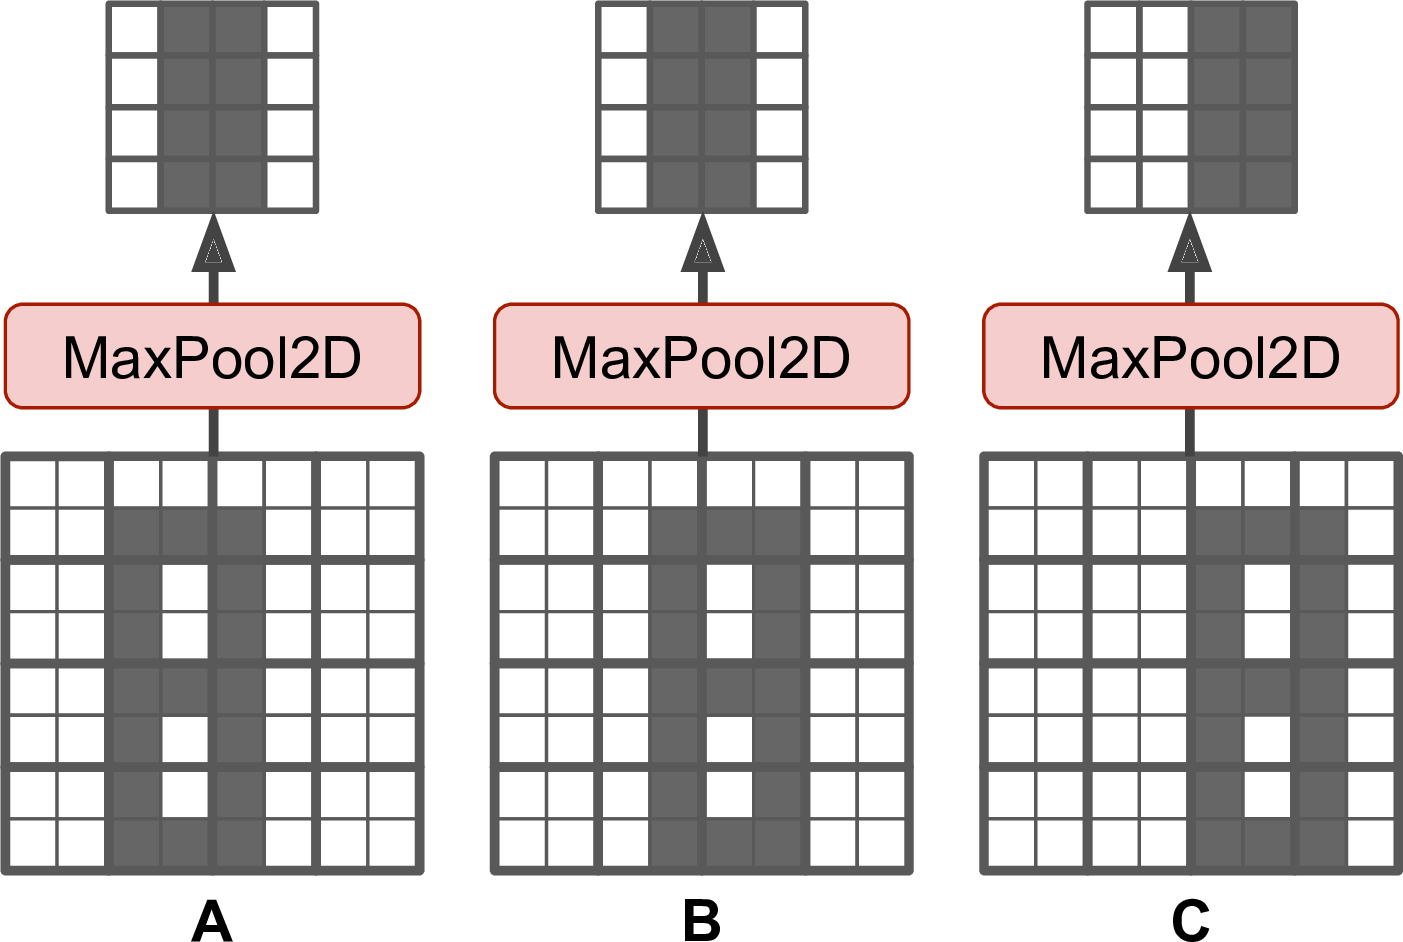
\includegraphics[width=.8\textwidth]{max_pooling_invariance.png}
    \end{center}
    \caption{Max pooling layer's invariance to small translations. Source: \cite{geron2019hands}.}
  \end{figure}

  The typical CNN architecture involves the aforementioned convolutional layers, pooling layers, and fully connected layers.
  Some well-established CNN architecutres are LeNet-5 \cite{lecun1998gradient}, AlexNet \cite{krizhevsky2012imagenet},
  GoogLeNet \cite{szegedy2015going}, VGGNet \cite{simonyan2014very}, ResNet (Residual Network) \cite{he2016deep}, Xception
  (Extreme Inception) \cite{chollet2017xception}, MobileNet \cite{howard2017mobilenets, sandler2018mobilenetv2},
  and SENet (Squeeze-and-Excitation Network) \cite{hu2018squeeze}.

  \begin{figure}[ht]
    \begin{center}
      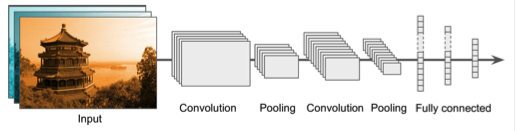
\includegraphics[width=.8\textwidth]{typical_cnn.png}
    \end{center}
    \caption{The typical CNN architecuture. Source: \cite{geron2019hands}.}
  \end{figure}

  Here we give ResNet a more in-depth introduction, as it's the backbone network of the model we use to detect amphoras.
  Resnet adds skip connections (or shortcut connections), which means the input signal of a layer is also added to the
  ouput of a higher up layer \cite{geron2019hands, he2016deep}. Skip connections help speed up the training considerably,
  since: 1) the network preconditions the problem to be the identify function, which is often close to the target function,
  and 2) the network can start making progress even if some layers have not started learning yet
  \cite{geron2019hands, he2016deep}. Batch normalization \cite{ioffe2015batch} is used after each convolution, which
  zero-centers and normalizes each input to reduce the vanishing gradient problem \cite{hochreiter1998vanishing} and the
  need for other regularization techniques like dropout \cite{srivastava2014dropout} \cite{geron2019hands, he2016deep}.
  The global average pooling layer at the end of the network is another type of pooling layer that gets the mean of the
  entire feature map \cite{geron2019hands, he2016deep}. Softmax is used in the output layer to ensure that all
  probabilities add up to 1 \cite{geron2019hands, he2016deep}.

  \begin{figure}[ht]
    \begin{center}
      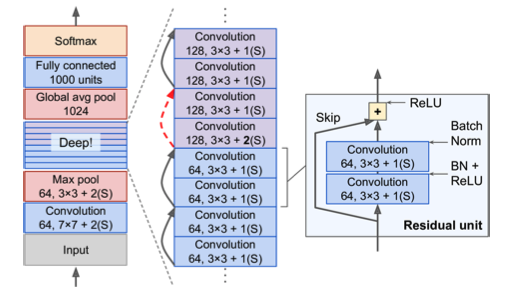
\includegraphics[width=.8\textwidth]{resnet.png}
    \end{center}
    \caption{ResNet architecture. Source: \cite{geron2019hands}.}
  \end{figure}

  \subsection{Deep Learning vs. Traditional Computer Vision}

  The increasingly abundant visual data and the improvements of deep learning algorithms, computing power, and image
  resolution have enabled deep learning to achieve state-of-the-art performance in many computer vision tasks, including
  image classification, object detection, and semantic segmentation \cite{qin2015underwater, voulodimos2018deep, o2019deep}.

  Traditionally, computer vision requires the manual feature selection and engineering step, which relies on domain knowledge
  to produce high-quality features \cite{elgendy2020deep, zhao2019object, o2019deep}. These handcrafted features are further
  procesed by a machine learning classifier like a support vector machine (SVM)
  \cite{elgendy2020deep, zhao2019object, o2019deep}. However, manual feature extraction becomes more and more complex as
  the number of classes increases \cite{o2019deep}. Besides, conventional machine learning algorithms' ability to
  generalize saturates quickly as the size of training data grows \cite{qin2015underwater}.

  In deep learning, the manual feature extraction step is no longer needed, and neural networks can be trained end-to-end
  as a feature extractor plus a classifier \cite{elgendy2020deep, o2019deep}. Thus, deep learning requires less domain
  knowledge, it and provides more flexibility as the models can be re-trained with a custom dataset for any specific use
  case \cite{o2019deep}.

  \begin{figure}[ht]
    \begin{center}
      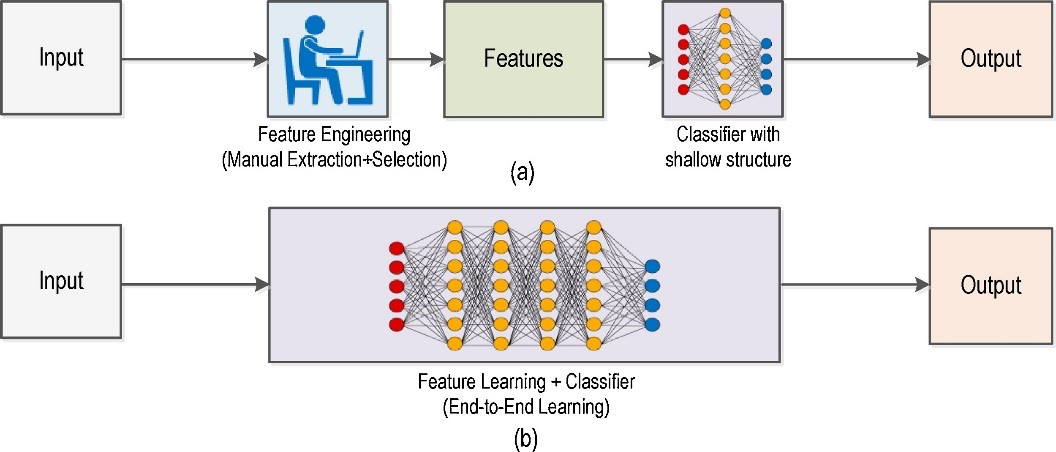
\includegraphics[width=.8\textwidth]{deep_learning_vs_traditional_computer_vision.png}
    \end{center}
    \caption{(a) Traditional computer vision workflow. (b) Deep learning workflow. Source: \cite{o2019deep}.}
  \end{figure}

  However, deep learning does not make traditional computer vision obsolete. Techniques like Scale Invariant Feature Transform
  (SIFT) \cite{karami2017image}, Speeded Up Robust Features (SURF) \cite{bay2006surf}, and Features from Accelerated
  Segment Test (FAST) \cite{rosten2006machine} are still useful in improving performance for computer vision tasks
  \cite{o2019deep}. And deep learning's performance depends on obtaining large datasets with high image resolution \cite{o2019deep}.
  Some popular public datasets like PASCAL Visual Object Classes (VOC) \cite{everingham2010pascal}, ImageNet
  \cite{russakovsky2015imagenet}, and Microsoft Common Objects in Context (COCO) \cite{lin2014microsoft}
  have respectively 500 thousand, 14 million, and 328 thousand images.

  \subsection{Object Detection}

  Object detection is the computer vision task that localizes and classifies objects in an image
  \cite{elgendy2020deep, zhao2019object, liu2020deep, geron2019hands}. Object detection remains to be one of the most
  challenging problems in computer vision, as it can be considered as both a regression task (localization by predicting
  the bounding box) and a classification task (predicting the object class in each bounding box)
  \cite{elgendy2020deep, girshick2014rich, geron2019hands}. Plus, the large variantions in viewpoints, poses, occlusions,
  and lighting conditions make it even more difficult to perform perfect object detection
  \cite{zhao2019object, liu2020deep}.

  The traditional sliding window approach is to train a CNN to classify and locate a single object, and then slide it
  across the image \cite{geron2019hands, pasquet2017amphora, girshick2014rich, redmon2016you}. This approach slides the
  CNN mulitple times with different window sizes to detect objects with various sizes, which causes it to be quite slow
  \cite{geron2019hands}.

  \begin{figure}[ht]
    \begin{center}
      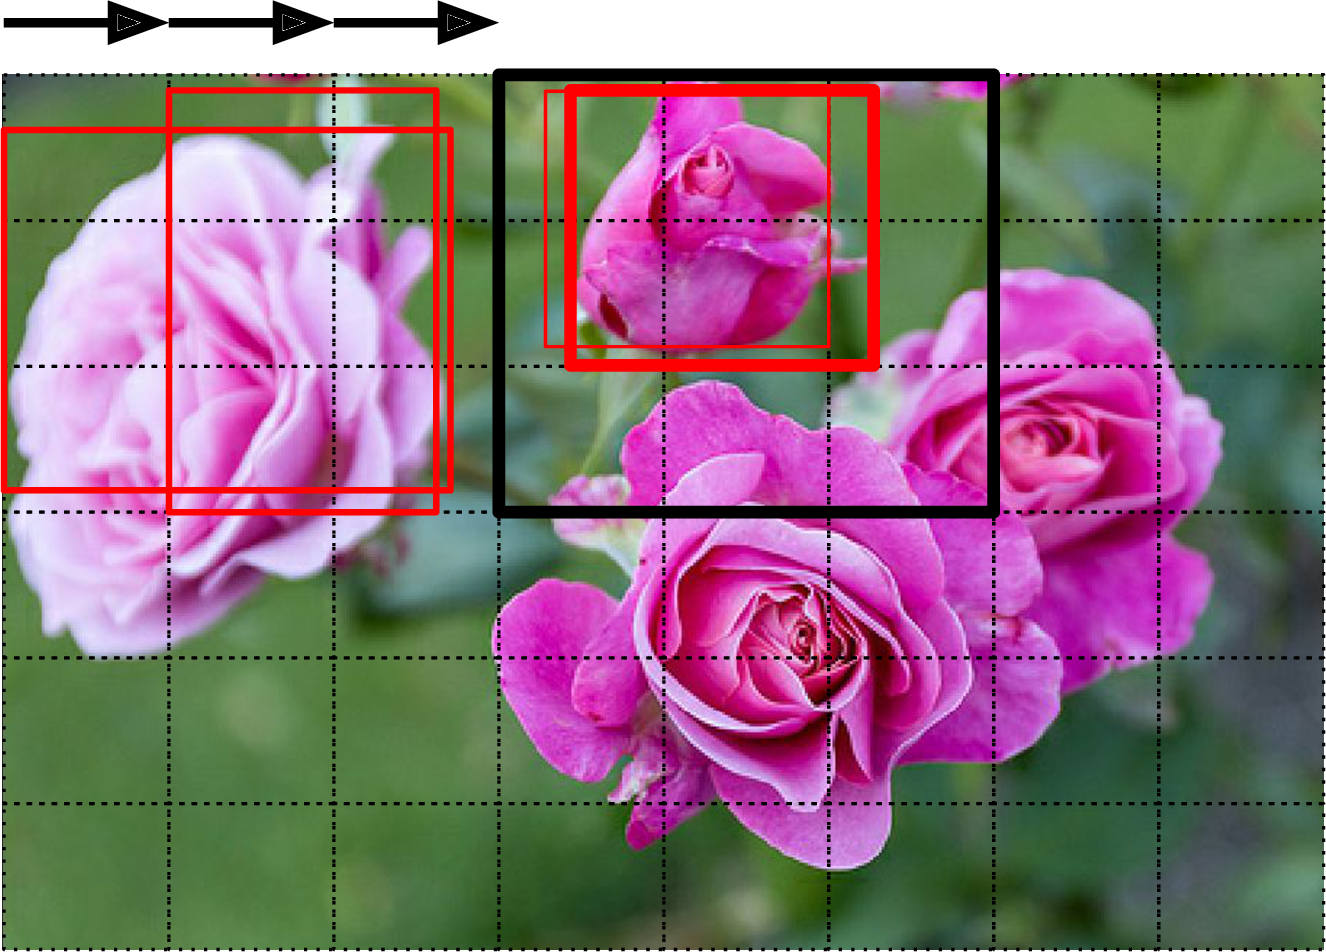
\includegraphics[width=.8\textwidth]{sliding_window.png}
    \end{center}
    \caption{The sliding window approach for object detection. Source: \cite{o2019deep}.}
  \end{figure}

  Luckily, many object detection frameworks based on fully convolutional network (FCN) \cite{long2015fully} have been
  introduced. FCNs contain only convolutional layers and pooling layers and only need to process each image once, which
  means they are faster and the input images can have arbitrary sizes \cite{elgendy2020deep, geron2019hands, long2015fully}.
  Here we summarize three well-established and influential object detection framework families: Region-Based Convolutional
  Neural Networks (R-CNN) \cite{girshick2014rich, girshick2015fast, ren2015faster}, Single Shot Detector (SSD)
  \cite{liu2016ssd}, and You Only Look Once (YOLO)
  \cite{redmon2016you, redmon2017yolo9000, redmon2018yolov3, bochkovskiy2020yolov4, yolov5}.

  \subsubsection{General Object Detection Framework Components}

  Before we dive into specific object detection frameworks, it's worth understanding the four high-level components of
  general object detection frameworks \cite{elgendy2020deep}.

  \paragraph{Region Proposal}

  The region proposal algorithm finds regions of interest (RoIs) that are further processed by the framework by
  discarding regions with low objectness score \cite{elgendy2020deep}. The objectness score indicates the probability of
  the region containing an object instead of the background, and it is the class probability for a single-class object
  detection task \cite{elgendy2020deep}.

  \paragraph{Network Predictions}

  A pretrained CNN is used as the backbone for feature extraction and makes the bounding-box prediction and class prediction
  for each region \cite{elgendy2020deep}. The bounding-box prediction is the tuple $(x, y, w, h)$, where $x$ and $y$ are
  the coordinates of the center and $w, h$ are the width and the height \cite{elgendy2020deep}.

  \paragraph{Non-Maximum Suppression (NMS)}

  The backbone network typically produces mulitple overlapping bounding boxes for one object, thus NMS finds
  the box with the maximum class probability and suppresses the rest \cite{elgendy2020deep}. The steps include
  \cite{elgendy2020deep}:

  \begin{enumerate}
    \item Discard boxes with predictions less than the tunable confidence threshold.
    \item Select the box with the highest probability.
    \item Compute the overlap - intersection over union (IoU) - of the boxes that have the same class prediction.
    Boxes with high IoU are averaged together.
    \item Suppress boxes with an IoU less than the tunable NMS threshold.
  \end{enumerate}

  \begin{figure}[ht]
    \begin{center}
      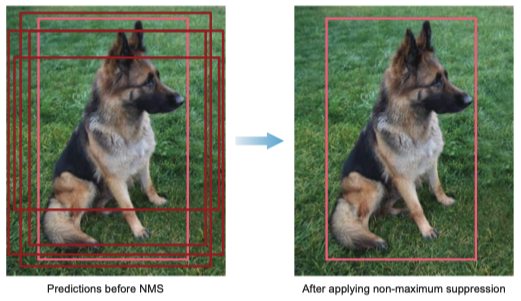
\includegraphics[width=.8\textwidth]{nms.png}
    \end{center}
    \caption{NMS. Source: \cite{elgendy2020deep}.}
  \end{figure}

  \paragraph{Metrics}

  The two main metrics for object detection are frames per second (FPS) and mean average precision (mAP)
  \cite{elgendy2020deep, liu2020deep, geron2019hands, planche2019hands}. To understand mAP, we need to understand first
  the aforementioned intersection over union (IoU) and the precision-recall curve (PR curve). The IoU is also known as
  the Jaccard index, which is used to messaure similarity between two sets \cite{planche2019hands}. The IoU can be
  mathematically formulated as follows \cite{elgendy2020deep, planche2019hands}:

  $$IoU = \frac{B_{ground \ truth} \cap B_{prediction}}{B_{ground \ truth} \cup B_{prediction}}$$

  \begin{figure}[ht]
    \begin{center}
      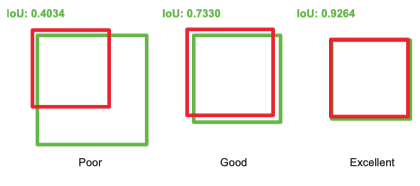
\includegraphics[width=.8\textwidth]{iou.png}
    \end{center}
    \caption{IOU. Source: \cite{elgendy2020deep}.}
  \end{figure}

  We say that the prediction is a true positive (TP) if the predicted class is the same as the ground truth and the IoU
  value is more than the tunable threshold, otherwise it is a false positive (FP)
  \cite{liu2020deep, elgendy2020deep, planche2019hands}. A false negative (FN) is a ground truth that does not have a
  prediction \cite{planche2019hands}. Then we can define precision and recall as follows
  \cite{burkov2019hundred, davis2006relationship}:

  $$Precision = \frac{TP}{TP + FP}$$

  $$Recall = \frac{TP}{TP + FN}$$

  \begin{figure}[ht]
    \begin{center}
      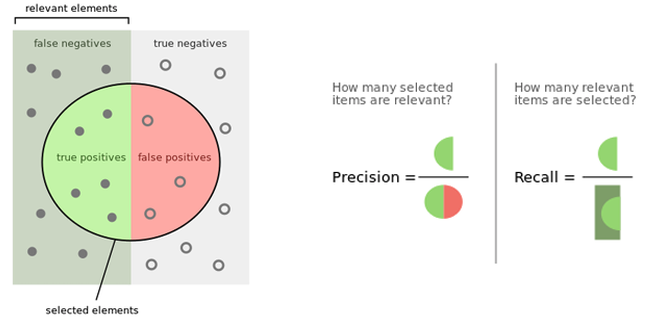
\includegraphics[width=.8\textwidth]{precision_recall.png}
    \end{center}
    \caption{Precision and recall. Source: \cite{precisionrecall}.}
  \end{figure}

  There is a trade-off between precision and recall
  \cite{elgendy2020deep, geron2019hands, burkov2019hundred, planche2019hands}. We can obtain the average precision
  (AP) by drawing the precision-recall curve (PR curve) and computing the area under the curve (AUC)
  \cite{elgendy2020deep, planche2019hands}. Finally, we get the mean average precision (mAP) by averaging
  the AP over all the classes \cite{elgendy2020deep, geron2019hands, planche2019hands}. Note that the AP and mAP are the
  same when it's a single-class object detetction task. The Pascal VOC metric uses mAP@0.5, which means the IOU threshold
  is 0.5 \cite{liu2020deep, everingham2010pascal, planche2019hands}. And the MS COCO metric - the one we are using for
  detecting amphoras - $mAP_{coco} = mAP@[0.50:0.05:0.95]$ is averaged with different IOU thresholds from 0.5 to 0.95 in
  steps of 0.05, which rewards detectors with better localization \cite{liu2020deep, planche2019hands, cocometrics}. MS
  COCO also introduces mAP for different scales: $mAP^{small}$ for small objects with area smaller than $32^2$ pixels,
  $mAP^{medium}$ for medium objects with area bigger than than $32^2$ pixels and smaller than $96^2$ pixels, and
  $mAP^{big}$ for big objects with area bigger than $96^2$ pixels \cite{liu2020deep, cocometrics}.

  \begin{figure}[ht]
    \begin{center}
      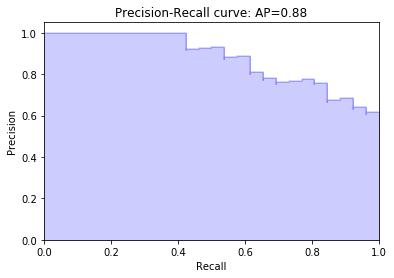
\includegraphics[width=.8\textwidth]{pr_curve.png}
    \end{center}
    \caption{A PR curve with 0.88 AUC. Source: \cite{planche2019hands}.}
  \end{figure}

  \subsubsection{Region-Based Convolutional Neural Networks (R-CNN)}

  The evolution from the original R-CNN \cite{girshick2014rich} to Fast R-CNN \cite{girshick2015fast} and then to
  Faster R-CNN \cite{ren2015faster} builds up the R-CNN family.

  \paragraph{R-CNN}

  R-CNN has four components \cite{elgendy2020deep, girshick2014rich}:

  \begin{enumerate}
    \item Region proposal with a greedy search algorithm called selective search, which finds RoIs by combining similar
    pixels into boxes.
    \item Feature extractor with a pretrained CNN.
    \item Classification with a linear SVM.
    \item Localization with a bounding-box regressor.
  \end{enumerate}

  \begin{figure}[ht]
    \begin{center}
      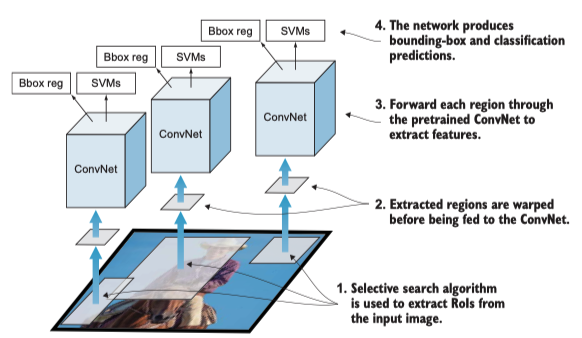
\includegraphics[width=.8\textwidth]{r_cnn.png}
    \end{center}
    \caption{R-CNN. Source: \cite{elgendy2020deep}.}
  \end{figure}

  R-CNN has the following disadvantages \cite{elgendy2020deep, girshick2014rich, girshick2015fast}:

  \begin{itemize}
    \item The FPS is very low. The selective search algorithm proposes about 2000 RoIs, which is every computationally
    expensive as the CNN has to process each proposal separately.
    \item The training is multi-stage, inelegant, expensive, and not end-to-end. It involves training three components
    separately: the CNN, the SVM, and the bounding-box regressor.
  \end{itemize}

  \paragraph{Fast R-CNN}

  Fast R-CNN makes the following changes from R-CNN \cite{elgendy2020deep, girshick2015fast}:

  \begin{itemize}
    \item The CNN goes before region proposal instead of after, so that the image only goes through the CNN once instead
    of 2000 RoIs going through the CNN separately.
    \item Classification is done by the softmax layer of the CNN instead of the SVM. And localization is also an output
    layer of the CNN.
    \item A RoI max pooling layer is added after region proposal to fix the input size for the fully connected layers.
    \item A multi-task loss function is used.
  \end{itemize}

  \begin{figure}[ht]
    \begin{center}
      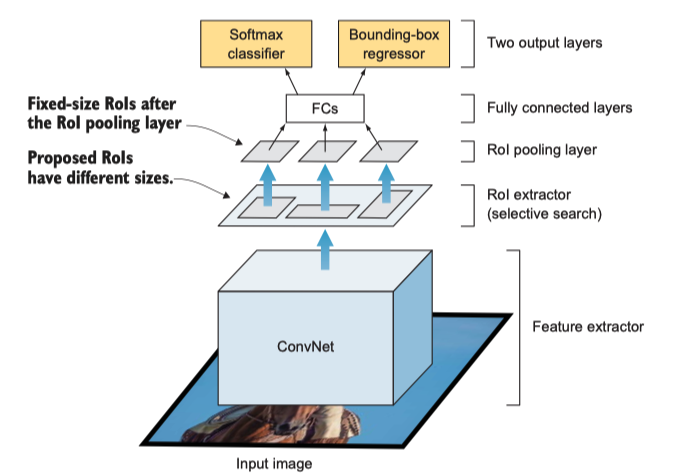
\includegraphics[width=.8\textwidth]{fast_r_cnn.png}
    \end{center}
    \caption{Fast R-CNN. Source: \cite{elgendy2020deep}.}
  \end{figure}

  Fast R-CNN is much faster than R-CNN, although the selective search algorithm still exists as the bottleneck
  \cite{elgendy2020deep, girshick2015fast, ren2015faster}.

  \paragraph{Faster R-CNN}

  Faster R-CNN makes the following improvments from Fast R-CNN \cite{elgendy2020deep, ren2015faster}:

  \begin{itemize}
    \item Region Proposal Network (RPN) or attention network replaces selective search, which reduces the number of
    proposals, speeds up the model, and makes the model training end-to-end. RPN is a FCN that outputs objectness scores
    and RoIs, and it can be used as a standalone network for single-class object detection. It also shares the features
    with the detection network, which enables region proposal to be nearly cost-free.
    \item Anchors are introduced as reference boxes at different scales and aspect ratios. Thus the regression layer
    only needs to output the offsets of coordinates, width, and height from the anchors. The anchors are created using
    the sliding-window approach. By default 9 anchors (3 scales and 3 aspect ratios) centered at each sliding window are
    created for each window.
  \end{itemize}

  \begin{figure}[ht]
    \begin{center}
      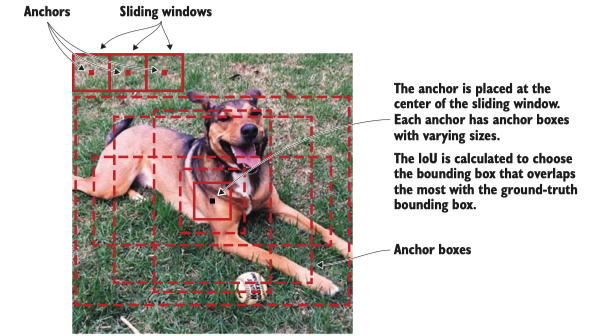
\includegraphics[width=.8\textwidth]{anchors.png}
    \end{center}
    \caption{Anchors in Faster R-CNN. Source: \cite{elgendy2020deep}.}
  \end{figure}

  \begin{figure}[ht]
    \begin{center}
      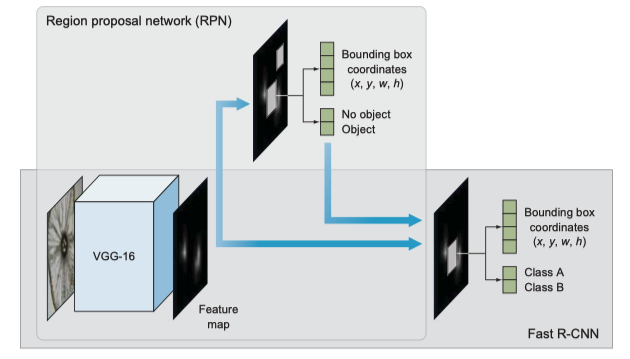
\includegraphics[width=.8\textwidth]{faster_r_cnn.png}
    \end{center}
    \caption{Faster R-CNN. Source: \cite{elgendy2020deep}.}
  \end{figure}

  To summarize, the R-CNN family are two-stage detectors that separate region proposal and detection \cite{elgendy2020deep}.
  They can not achieve real-time detection (only 7 FPS), and they are too computationally intensive
  \cite{elgendy2020deep, liu2016ssd, redmon2016you}. One-stage detectors like Single Shot Detector (SSD) and You Only
  Look Once (YOLO) skip the region proposal to achieve real-time detection speed \cite{elgendy2020deep}. In general,
  one-stage detectors sacrifices some accuracy for speed \cite{elgendy2020deep, lin2017focal}.

  \subsubsection{Single Shot Detector (SSD)}

  Single Shot Detector (SSD) makes both the objectness and class probability predictions directly in one shot
  \cite{elgendy2020deep, liu2016ssd}. It has three main components \cite{elgendy2020deep, liu2016ssd}:

  \begin{itemize}
    \item The base network, which is VGG-16 in the original paper. It also uses anchors called priors like in Faster R-CNN.
    But the network sends the bounding box offsets and the class scores to NMS directly when it finds a bounding box that
    contains the object features.
    \item Multi-scale feature layers, which are convolutional layers that decrease in size progressively to detect objects
    at multiple scales. The resolution of feature maps decreases as the CNN reduces the spatial dimension.
    \item NMS.
  \end{itemize}

  \begin{figure}[ht]
    \begin{center}
      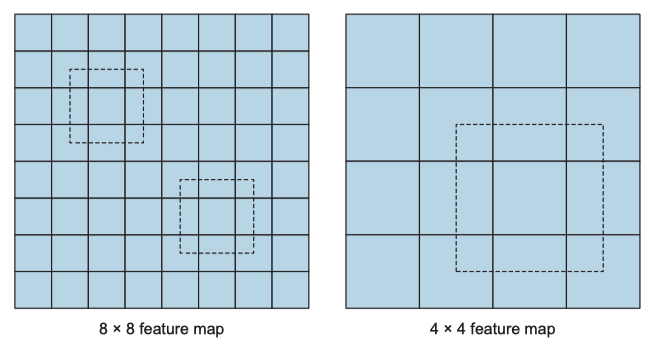
\includegraphics[width=.8\textwidth]{ssd_feature_maps.png}
    \end{center}
    \caption{Multi-scale feature maps in SSD. Higher-resolution feature maps (left) detect smaller objects.
    Lower-resolution feature mpas (right) detect bigger objects Source: \cite{elgendy2020deep}.}
  \end{figure}

  \begin{figure}[ht]
    \begin{center}
      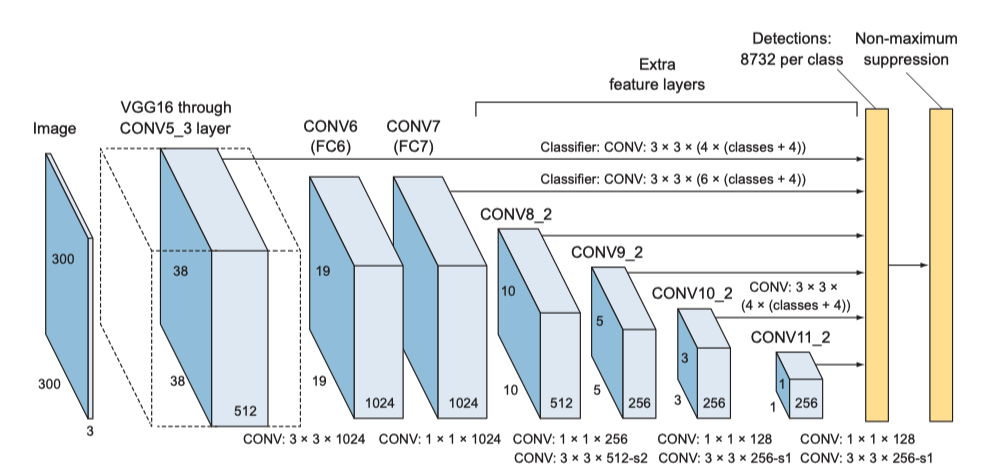
\includegraphics[width=.8\textwidth]{ssd.png}
    \end{center}
    \caption{SSD. Source: \cite{elgendy2020deep}.}
  \end{figure}

  In short, SSD300 (300 x 300 input size) is able to achieve real-time detection with 59 FPS, while SSD512 outperforms
  Faster R-CNN in terms of mAP \cite{liu2016ssd}.

  \subsubsection{You Only Look Once (YOLO)}

  Like the R-CNN family, the YOLO family has been going through a series of improvements since the original YOLO paper
  was published. YOLO is also a one-stage real-time detector simlar to SSD. YOLOv1 \cite{redmon2016you} introduces the
  general architecture; YOLOv2 \cite{redmon2017yolo9000} adds anchors similar to Faster R-CNN and SSD; YOLOv3
  \cite{redmon2018yolov3} further refines the architecture and the training process; YOLOv4 \cite{bochkovskiy2020yolov4}
  makes use of some universal object detector features called "bag of freebies" and "bag of specials"; YOLOv5 \cite{yolov5}
  is under active development and authors have yet to publish a paper.

  YOLO divides the image into a grid, and a grid cell is responsible for detecting an object if the center of the object
  is inside the cell \cite{elgendy2020deep, redmon2016you}. The backbone network is called DarkNet, which is inspired by
  GoogLeNet \cite{elgendy2020deep, redmon2016you}.

  \begin{figure}[ht]
    \begin{center}
      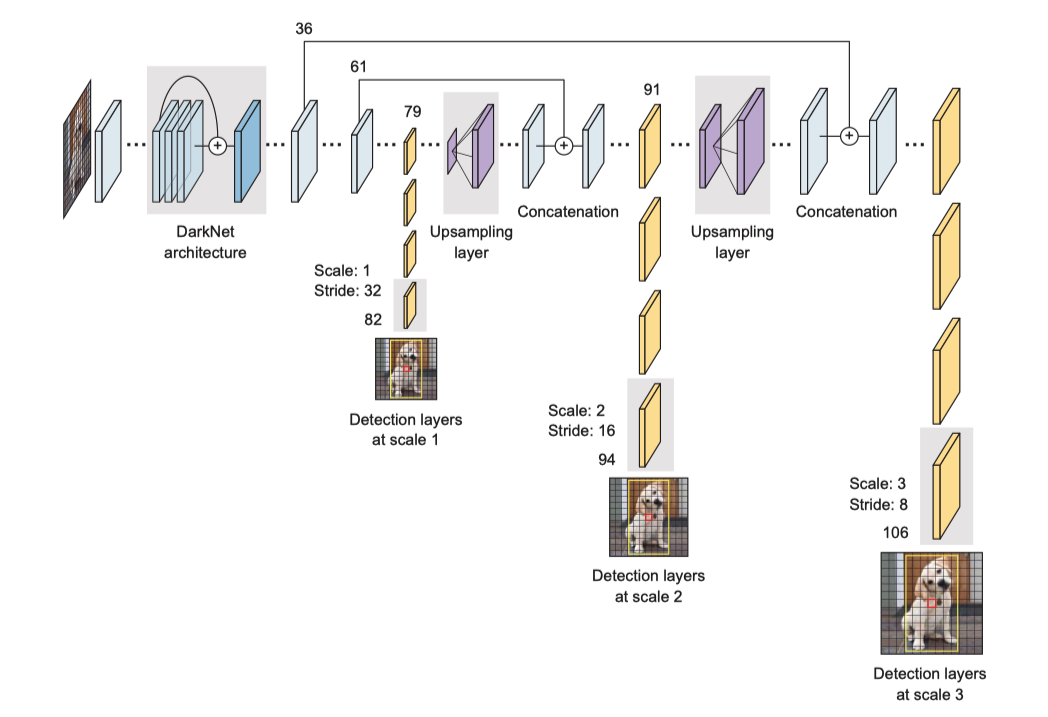
\includegraphics[width=\textwidth]{yolov3.png}
    \end{center}
    \caption{YOLOv3 architecture. YOLO performs detections at 3 different scales. Layer 79 makes a grid of 13 x 13 to
    detect large objects. Layer 91 makes a grid of 26 x 26 to detect medium objects. And finally layer 106 makes a grid
    of 52 x 52 to detect small objects. Source: \cite{elgendy2020deep}.}
  \end{figure}

  YOLOv4, a bleeding-edge detector introduced in 2020, utilizes numerous new features to improve the performance
  from YOLOv3, including DropBlock regulariztion \cite{ghiasi2018dropblock}, Mish activation \cite{misra2019mish},
  Self-Adversarial Training \cite{bochkovskiy2020yolov4}, etc.

  \section{Related Work}

  As we have mentioned in \hyperref[sec:112]{section 1.1.2}, there is limited research on the application of deep learning
  for underwater archaeology and vision-based underwater object detection in general.

  For fish detection, Qin et al. \cite{qin2015underwater, li2015fast}, Zhang et al. \cite{zhang2016unsupervised},
  Villon et al. \cite{villon2016coral}, Xu et al. \cite{xu2018underwater}, and Konovalov et al.
  \cite{konovalov2019underwater} respectively use Fast R-CNN, a model similar to R-CNN, sliding window with a CNN,
  YOLOv3, and Xception.

  For crab detection, Can et al. \cite{cao2020real} proposes a detector called Faster MSSDLite, which is based on SSD with
  a MobileNetv2 backbone and feature pyramid network (FPN) \cite{lin2017feature}.

  For planktons and corals, we have only found research for classification but not object detection
  \cite{qin2015underwater, moniruzzaman2017deep}.

  For amphora detection, Pasquet et al. \cite{mccarthy20193d, pasquet2017amphora} uses sliding window with a CNN on
  high-resolution orthophotos (aerial photos). And this is the only study we have found on amphora detection with deep
  learning.

  \section{Data and Methods}

  \subsection{Data}

  The dataset consists of 50 images (294 objects) in the training set and 7 images (31 objects) in the validation set,
  which maintains the 90\% : 10\% ratio for the object count. Two additional images are used as the test set. All the
  images are obtained through various sources \cite{googleimages, groplan, phoenician} and are annotated with LabelImg
  \cite{labelimg}.

  \subsection{Model}
  % UAV require real-time
  \subsection{Model Training}

  \section{Evaluation}

  This section discusses criteria that are used to evaluate the
  research results. Make sure your results can be used to published
  research results, i.e., to the already known state-of-the-art.

  (target size: 5-10 pages)

  \begin{table}[ht]
    \begin{center}
      \begin{tabular}{cl}
        \toprule
        Number & Description \\
        \midrule
        7 & A lucky number in Western culture \\
        8 & A lucky number in Chinese and other Asian cultures \\
        42 & Answer to the ultimate question of life, the universe, and everything \\
        404 & Not found \\
        \bottomrule
      \end{tabular}
      \caption{Useless insights I gained with no further meaning}
    \end{center}
  \end{table}

  \subsection{Visual Evaluation}
  \subsection{Metric Evaluation}

  \section{Conclusions}

  Summarize the main aspects and results of the research
  project. Provide an answer to the research questions stated earlier.

  (target size: 1/2 page)

  \section{Future Work}
  % \cite{mccarthy20193d,pasquet2017amphora} define three classes as amphoras are often broken

  \newpage

  \printbibliography

\end{document}
